\section{Charging and Discharging Capacitors (RC circuits)}

\begin{comment}
This lab was originally written by Matt Trawick in around 2008, and finally transcribed to Latex for inclusion in this lab manual in 2015.  This lab builds on "Introduction to Electric Circuits" and uses a lot of the same pedagogical approaches, but can be used independently.

IMHO, this lab is flat out much better than the existing lab, titled ``RC circuits,'' for lots of reasons:
1. The old lab relies on the internal resistance of analog voltmeters, about 3000 ohms.  This makes it hard for students to see and understand what R actually is, since the meter is a meter first, and a resistor only secondarily.  Using the meter also makes it harder to change R, and the old lab never has students test different resistor values. This new lab uses actual resistors for the job.  (Besides, using analog voltmeters is insanity; nobody outside UR has used them since the Nixon administration.)

2. The old lab uses only one capacitor, so students never see how the time constant depends on C.

3. Pedagogically, the old lab starts with equations, whereas the new lab starts with pictures of circuits and qualitative questions, before working up to an equation for a discharging capacitor at the end of the lab.

4. The new lab explicitly has students make qualitative predictions, and then test them.  The old lab does not.

5.  The old lab talks about the ``half-life'' of an RC circuit.  ``half life'' is used for nuclear decay, but is basically never used for RC circuits in the real world.

In summary, the old ``RC circuits'' lab should be removed, and replaced with this one.

When I teach this lab, I usually wait until students are finished with activity 1 (so they've seen charging and discharging with their own eyes, so to speak) before I launch into a quick refresher lecture about what's happening, and how charge is going through the resistor and building up on one side of the capacitor, but charge is draining away from the other side, and so on.  This is also where I use a water analogy, where the battery is a pump, the resistor is a constriction in the pipe, and the capacitor is a place where the pipe gets wide, and a rubber membrane is stretched across it.

As with any lab, some students finish quickly, some not so much.  I generally cut off the lab when the slowest students have finished part 2(g).  Some students will have figured out on their own that V(t) is a decaying exponential, and some won't have.  I'm okay with that; I'll talk about it in a lecture for those who didn't get there on their own.

Equipment notes: 

I believe the circuits here are most easily (and intuitively) constructed using banana cables, which means that the resistors and capacitors should all be mounted ahead of time into dual banana socckets.  DPST knife switches should also have banana jacks attached to them.  

The values of resistors and capacitors used here are not an accident.  The RC time constants used are slow enough to be easily visible and measurable by the students.  Also, the resistance values are low enough that they are safely below the ~1 Mohm input impedance of the pasco 750 boxes.   That pushes the capacitors to fairly high values, and you can run into troubles there if the capacitors have a high leakage current.  For this reason, it's important to use capacitors with a reasonably low leakage.  
\end{comment}

\makelabheader %(Space for student name, etc., defined in master.tex)

\vspace{0.1in}
\textbf{Apparatus} 
\begin{itemize}%[nolistsep]
\setlength\itemsep{-4pt}
\setlength\topsep{-6pt}
\setlength\partopsep{-6pt}
\vspace{-0.2in}  %There's gotta be a better way to tame this list spacing than this!  --MT
\item Digital multimeter 
\item DC power supply 
\item Pasco 750 interface, with voltage leads
\item Resistors: 10 k$\Omega$ and 27 k$\Omega$
\item Capacitors: 470 $\mu$F and 1000 $\mu$F (``low leakage'')
\item 4 dual banana connectors for resistors and capacitors
\item DPST knife switch with banana jack connectors (optional)
\item About six connecting wires
\end{itemize}

\textbf{Activity 1}

Build the circuit shown in the diagram below.  If you do not have an actual switch, then you can accomplish the same thing by plugging and unplugging wires as needed.

\begin{minipage}{0.83\textwidth}
\begin{newboxed}
\vspace{-0.2 in}
\textit{Be sure to connect the “negative” end of the capacitor to the negative terminal of the power supply, or it may explode and hurt you.  The negative terminal is marked with a long stripe down the side of the capacitor with negative signs (``$-$'') on it.  In the figure to the right, the upper wire is the negative terminal. Ask your instructor for help if you are not sure.}
\vspace{-0.1 in}
\end{newboxed}
\end{minipage}
\begin{minipage}{0.17\textwidth}
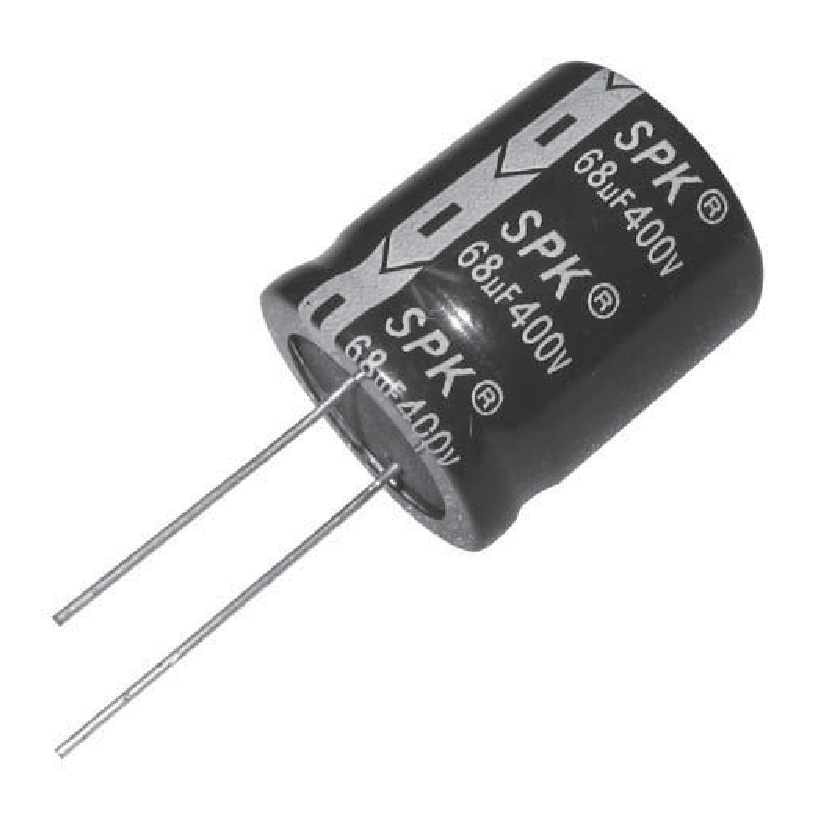
\includegraphics[width=1.0\textwidth]{rc_circuits/capacitor_bw.eps}
\end{minipage}

\begin{center}
\vspace{-0.3 in}
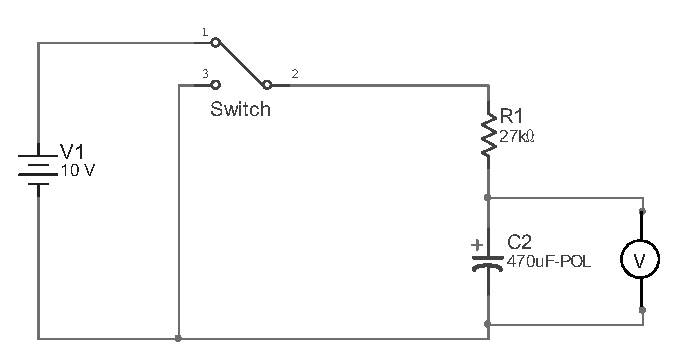
\includegraphics[width=0.6\textwidth]{rc_circuits/circuit_diagram_bw.eps}
\vspace{-0.2 in}
\end{center}

(a) When you move the switch to position ``1'' as shown, so that terminals 1 and 2 are connected, what happens to the voltage difference $\Delta V_C$ across the capacitor?
\vspace{0.6in}

(b)  With the switch in position ``1'' as shown, what is happening to the charge $Q$ stored on the capacitor?
\vspace{0.6in}

(c)  Now move the switch to position ``3,'' so that terminals 1 and 2 are connected.  What happens to the voltage difference $\Delta V_C$ and the charge $Q$ on the capacitor?
\vspace{0.8in}

\pagebreak
\textbf{Activity 2}

Because the voltage $\Delta V_C$ is changing, it will be useful to use your computer to graph $\Delta V_C$ \textit{vs.} time.  Put the two red and black leads from the 750 interface box where your digital voltmeter is connected to your circuit.  (You can keep the DMM plugged in too.)

To record voltage versus time data, go to \textit{Start $\longrightarrow$ Programs $\longrightarrow$ PhysicsApplications $\longrightarrow$ Datastudio}. Select the option Create Experiment.  You will see an image of the 750 interface box.  On this image, click on the channel A input.  You will see a list of sensors.  Scroll down to the Voltage Sensor and select by clicking OK.  Finally open a graph display by double clicking on the Graph option (on the left).

(a)  Now take some data.  Draw sketches below showing $\Delta V_C$ \textit{vs.} time when the switch is moved into position ``1'' (charging) and position ``3'' (discharging).
\vspace{1.5in}

(b)  Helpful hint: if you get tired of waiting forever for $\Delta V_C$ to rise and fall, you can briefly “short out” the resistor by connecting an additional wire across it, like this.  
\begin{center}
\vspace{-0.2 in}

\includegraphics[width=0.05\textwidth]{rc_circuits/shorted_resistor_bw.eps}
\vspace{-0.2 in}
\end{center}
How does “shorting out” the resistor affect $\Delta V_C$ when the capacitor is charging?  When the capacitor is discharging?
\vspace{0.8in}

(c) Start with the capacitor fully charged at about 10 volts.  Then (with the resistor not shorted out) move the switch to position “3” to discharge the capacitor.  How long does it take for $\Delta V_C$ to drop to 1/3 of its original level (that is, from 10 volts to about 3.3 volts)?
\vspace{0.8in}

(d) If you repeat part (c) with a resistance $R = 10$ k$\Omega$ how do you expect your result to change?  Make a prediction and then test it.

\vspace{0.2 in}
\hspace{0.4 in} Prediction:
\vspace{0.2 in}

\hspace{0.4 in} Measurement:  
\vspace{0.2 in}

\pagebreak
(e) Go back to using the 27 k$\Omega$ resistor.  Now, if you repeat part (c) with a capacitance of $C=1000$ $\mu$F, how do you expect your result to change?  Make a prediction and then test it.

\vspace{0.2 in}
\hspace{0.4 in} Prediction:
\vspace{0.2 in}

\hspace{0.4 in} Measurement:  
\vspace{0.2 in}

(f) The time it takes for $\Delta V_C$ to fall to about a third of its original value (actually to $1/e$ of its value, where $e=2.71828…$) is called the time constant, $\tau$.   Fill in the following table:

%For fixed width columns:
%These are now defined in master.text, to avoid  warnings when the definition is repeated in each file.
%columntype{L}[1]{>{\raggedright\arraybackslash}p{#1}}
%\newcolumntype{C}[1]{>{\centering\arraybackslash}p{#1}}
%\newcolumntype{R}[1]{>{\raggedleft\arraybackslash}p{#1}}

\vspace{0.1 in}
\renewcommand{\arraystretch}{1.8}
\hspace*{0.5in}
%\begin{tabular}{|c | c| >{\centering}m{1in} |}
\begin{tabular}{|c | c| C{1in} |}
\hline
$R$ & $C$ & $\tau$ \\ \hline
10 k$\Omega$ & 470 $\mu$F &\\ \hline
27 k$\Omega$ & 470 $\mu$F &\\ \hline
10 k$\Omega$ & 1000 $\mu$F &\\ \hline
27 k$\Omega$ & 1000 $\mu$F &\\ \hline
\end{tabular}
\renewcommand{\arraystretch}{1.0}
\vspace{0.3in}

(g) What is the relationship between $R$, $C$, and $\tau$?
\vspace{0.7in}

(h) Looking at your graphs, what is the functional form of $\Delta V_C$ \textit{vs.} time  for a discharging capacitor?  Try moving your data to Excel and fitting it to test your hypothesis.
\vspace{0.7in}
